% Options for packages loaded elsewhere
\PassOptionsToPackage{unicode}{hyperref}
\PassOptionsToPackage{hyphens}{url}
\PassOptionsToPackage{dvipsnames,svgnames,x11names}{xcolor}
%
\documentclass[
]{agujournal2019}

\usepackage{amsmath,amssymb}
\usepackage{iftex}
\ifPDFTeX
  \usepackage[T1]{fontenc}
  \usepackage[utf8]{inputenc}
  \usepackage{textcomp} % provide euro and other symbols
\else % if luatex or xetex
  \usepackage{unicode-math}
  \defaultfontfeatures{Scale=MatchLowercase}
  \defaultfontfeatures[\rmfamily]{Ligatures=TeX,Scale=1}
\fi
\usepackage{lmodern}
\ifPDFTeX\else  
    % xetex/luatex font selection
\fi
% Use upquote if available, for straight quotes in verbatim environments
\IfFileExists{upquote.sty}{\usepackage{upquote}}{}
\IfFileExists{microtype.sty}{% use microtype if available
  \usepackage[]{microtype}
  \UseMicrotypeSet[protrusion]{basicmath} % disable protrusion for tt fonts
}{}
\makeatletter
\@ifundefined{KOMAClassName}{% if non-KOMA class
  \IfFileExists{parskip.sty}{%
    \usepackage{parskip}
  }{% else
    \setlength{\parindent}{0pt}
    \setlength{\parskip}{6pt plus 2pt minus 1pt}}
}{% if KOMA class
  \KOMAoptions{parskip=half}}
\makeatother
\usepackage{xcolor}
\setlength{\emergencystretch}{3em} % prevent overfull lines
\setcounter{secnumdepth}{5}
% Make \paragraph and \subparagraph free-standing
\ifx\paragraph\undefined\else
  \let\oldparagraph\paragraph
  \renewcommand{\paragraph}[1]{\oldparagraph{#1}\mbox{}}
\fi
\ifx\subparagraph\undefined\else
  \let\oldsubparagraph\subparagraph
  \renewcommand{\subparagraph}[1]{\oldsubparagraph{#1}\mbox{}}
\fi


\providecommand{\tightlist}{%
  \setlength{\itemsep}{0pt}\setlength{\parskip}{0pt}}\usepackage{longtable,booktabs,array}
\usepackage{calc} % for calculating minipage widths
% Correct order of tables after \paragraph or \subparagraph
\usepackage{etoolbox}
\makeatletter
\patchcmd\longtable{\par}{\if@noskipsec\mbox{}\fi\par}{}{}
\makeatother
% Allow footnotes in longtable head/foot
\IfFileExists{footnotehyper.sty}{\usepackage{footnotehyper}}{\usepackage{footnote}}
\makesavenoteenv{longtable}
\usepackage{graphicx}
\makeatletter
\def\maxwidth{\ifdim\Gin@nat@width>\linewidth\linewidth\else\Gin@nat@width\fi}
\def\maxheight{\ifdim\Gin@nat@height>\textheight\textheight\else\Gin@nat@height\fi}
\makeatother
% Scale images if necessary, so that they will not overflow the page
% margins by default, and it is still possible to overwrite the defaults
% using explicit options in \includegraphics[width, height, ...]{}
\setkeys{Gin}{width=\maxwidth,height=\maxheight,keepaspectratio}
% Set default figure placement to htbp
\makeatletter
\def\fps@figure{htbp}
\makeatother
% definitions for citeproc citations
\NewDocumentCommand\citeproctext{}{}
\NewDocumentCommand\citeproc{mm}{%
  \begingroup\def\citeproctext{#2}\cite{#1}\endgroup}
\makeatletter
 % allow citations to break across lines
 \let\@cite@ofmt\@firstofone
 % avoid brackets around text for \cite:
 \def\@biblabel#1{}
 \def\@cite#1#2{{#1\if@tempswa , #2\fi}}
\makeatother
\newlength{\cslhangindent}
\setlength{\cslhangindent}{1.5em}
\newlength{\csllabelwidth}
\setlength{\csllabelwidth}{3em}
\newenvironment{CSLReferences}[2] % #1 hanging-indent, #2 entry-spacing
 {\begin{list}{}{%
  \setlength{\itemindent}{0pt}
  \setlength{\leftmargin}{0pt}
  \setlength{\parsep}{0pt}
  % turn on hanging indent if param 1 is 1
  \ifodd #1
   \setlength{\leftmargin}{\cslhangindent}
   \setlength{\itemindent}{-1\cslhangindent}
  \fi
  % set entry spacing
  \setlength{\itemsep}{#2\baselineskip}}}
 {\end{list}}
\usepackage{calc}
\newcommand{\CSLBlock}[1]{\hfill\break\parbox[t]{\linewidth}{\strut\ignorespaces#1\strut}}
\newcommand{\CSLLeftMargin}[1]{\parbox[t]{\csllabelwidth}{\strut#1\strut}}
\newcommand{\CSLRightInline}[1]{\parbox[t]{\linewidth - \csllabelwidth}{\strut#1\strut}}
\newcommand{\CSLIndent}[1]{\hspace{\cslhangindent}#1}

\usepackage{url} %this package should fix any errors with URLs in refs.
\usepackage{lineno}
\usepackage[inline]{trackchanges} %for better track changes. finalnew option will compile document with changes incorporated.
\usepackage{soul}
\linenumbers
\makeatletter
\@ifpackageloaded{caption}{}{\usepackage{caption}}
\AtBeginDocument{%
\ifdefined\contentsname
  \renewcommand*\contentsname{Table of contents}
\else
  \newcommand\contentsname{Table of contents}
\fi
\ifdefined\listfigurename
  \renewcommand*\listfigurename{List of Figures}
\else
  \newcommand\listfigurename{List of Figures}
\fi
\ifdefined\listtablename
  \renewcommand*\listtablename{List of Tables}
\else
  \newcommand\listtablename{List of Tables}
\fi
\ifdefined\figurename
  \renewcommand*\figurename{Figure}
\else
  \newcommand\figurename{Figure}
\fi
\ifdefined\tablename
  \renewcommand*\tablename{Table}
\else
  \newcommand\tablename{Table}
\fi
}
\@ifpackageloaded{float}{}{\usepackage{float}}
\floatstyle{ruled}
\@ifundefined{c@chapter}{\newfloat{codelisting}{h}{lop}}{\newfloat{codelisting}{h}{lop}[chapter]}
\floatname{codelisting}{Listing}
\newcommand*\listoflistings{\listof{codelisting}{List of Listings}}
\makeatother
\makeatletter
\makeatother
\makeatletter
\@ifpackageloaded{caption}{}{\usepackage{caption}}
\@ifpackageloaded{subcaption}{}{\usepackage{subcaption}}
\makeatother
\ifLuaTeX
  \usepackage{selnolig}  % disable illegal ligatures
\fi
\usepackage{bookmark}

\IfFileExists{xurl.sty}{\usepackage{xurl}}{} % add URL line breaks if available
\urlstyle{same} % disable monospaced font for URLs
\hypersetup{
  pdftitle={Diffusion Curvature for Fast, Point-wise, Noise-Resistant Geometric Featurization of Graphs and Pointclouds},
  pdfauthor={Kincaid MacDonald; Dhananjay Bhaskar; Kaly Zhang; Ian Adelstein; Smita Krishnaswamy},
  pdfkeywords={Manifold Learning, Geometric Deep Learning, Graph
Curvature, Point Clouds},
  colorlinks=true,
  linkcolor={blue},
  filecolor={Maroon},
  citecolor={Blue},
  urlcolor={Blue},
  pdfcreator={LaTeX via pandoc}}

\journalname{IEEE TPAMI}

\draftfalse

\begin{document}
\title{Diffusion Curvature for Fast, Point-wise, Noise-Resistant
Geometric Featurization of Graphs and Pointclouds}

\authors{Kincaid MacDonald\affil{1}, Dhananjay Bhaskar\affil{2}, Kaly
Zhang\affil{2}, Ian Adelstein\affil{3}, Smita Krishnaswamy\affil{4,5}}
\affiliation{1}{Yale, }\affiliation{2}{MILA, }\affiliation{3}{Yale
Department of Math, }\affiliation{4}{Yale Department of Applied
Math, }\affiliation{5}{Yale School of Medicine, }
\correspondingauthor{Kincaid MacDonald}{kincaid@aya.yale.edu}


\begin{abstract}
For a number of years now work has been proceeding in order to bring to
perfection the crudely conceived idea of a machine that would not only
supply inverse reactive current for use in unilateral phase detractors,
but would also be capable of automatically synchronizing cardinal
grammeters. Such a machine is the ``Turbo-Encabulator.''
\end{abstract}

\section*{Plain Language Summary}
We introduce Diffusion Curvature, a fast, differentiable, noise-robust
pointwise curvature for graphs and point clouds.



\section{Introduction}\label{introduction}

One of the most ubiquitous subjects of analysis in data science is the
humble point cloud. The points, by themselves, are high dimensional and
noisy; it is up to the data scientist to wring sense out of them. Per
the Manifold Hypothesis, we assume the points were sampled on or near
the surface of a low-dimensional manifold embedded in high-dimensional
Euclidean space. Manifold learning methods, like t-SNE, PHATE, and
Diffusion Maps
{[}(\textbf{maaten2008VisualizingDataUsing?}){]}(\textbf{moon2019VisualizingStructureTransitions?})(\textbf{coifman2006DiffusionMaps?}),
endeavor to recover salient features of the underlying manifold, like
geodesic distances, population clusterings, and dimension, from its
high-dimensional noisy sampling.

Curvature is a particularly troublesome geometric property to translate
into the discrete, sampled realm. In smooth Riemannian manifolds,
curvature is a \emph{local} phenomenon. It can be obtained by fitting
osculating circles of radius limiting to zero, or computed from the
manifold's Hessian, using the Second Fundamental Form. None of these
translate into the discrete realm. In a sampled manifold, taking a local
limit is impossible -- one can't ``zoom in'' past the sampling of points
-- and we don't have access to the parametrization of the manifold or
its tangent bundle, without computationally costly and potentially
error-prone estimation. Moreover, as our sampling is likely noisy, the
curvature can only be recovered over a sufficiently large neighborhood
of points to counter the spurious geometric artifacts created noisy
sampling. Thus, in the discrete realm, curvature becomes a
``semi-local'' phenomenon, in which neither the smallest nor larger
scales can be trusted.

There are elegant generalizations of classical curvature to discrete
spaces that overcome many of these roadblocks. Ollivier's \emph{Coarse
Ricci Curvature} (CRC) employs optimal transport theory to relate the
behavior of a discrete neighborhood to its smooth counterpart
(\textbf{ollivier2009RicciCurvatureMarkov?}). Sturm's \emph{displacement
convexity of entropy} (DCE) measures the proliferation of midpoints in
positive curvature (\textbf{sturm2006GeometryMetricMeasure?}). Both
methods use optimal transport as the basis of their ``semi-local''
measurement. Rather than trying to zoom in on a point, they define
curvature between pairs of points, approximating, at a coarse scale, a
Ricci tangent vector.

Although these techniques are theoretically elegant, general, and
applicable to any metric measure space, the setting of noisily sampled
point clouds is practically challenging for CRC and DCE. Both methods
rely on the graph's shortest-path lengths as an approximation of the
manifold's ground distance - a perilous assumption when dealing with
noisy data. And for large datasets, optimal transport calculations can
be computationally prohibitive.

In this paper, we develop Diffusion Curvature, a fast curvature estimate
derived solely from the graph diffusion matrix. We first introduced the
ideas behind Diffusion Curvature in
(\textbf{bhaskarDiffusionCurvatureEstimating2022?}), in which we
demonstrated its ability to produce an unsigned magnitude of curvature
estimation for toy datasets and single-cell data, and proved a
correspondence between the ratios of scalar curvature and diffusion
curvature. We now present a refined definition which produces
\emph{signed} curvature values and prove bounds relating Diffusion
Curvature to coarse Ricci Curvature. We demonstrate Diffusion
Curvature's robustness to noise and sampling artifacts, and position our
technique as an adaptation of coarse Ricci curvature particularly
suitable for point cloud data. \#\# Background

\subsection{Curvature in the Continuous
Setting}\label{curvature-in-the-continuous-setting}

\subsection{The Discrete Setting}\label{the-discrete-setting}

Within the ambient setting of points \(x_{i} \in \mathbb{R}^D\), the
Euclidean distances between the points in our point cloud are not very
useful. To perform geometric analysis, we want the manifold's
\emph{geodesic} distances between \(x_{i}, x_{j \in \mathcal{M}}\),.
However, manifolds are locally euclidean, so within a sufficiently small
neighborhood of \(x_{i} \in \mathcal{M}\) , the euclidean distances are
accurate. This is the basis of graph construction: retain only the
trustworthy local distances, discard the rest, and then ``integrate''
over the local neighborhoods to recover features of the global geometry.

A graph \(G = (V, E)\) is a collection of \(n\) vertices \(v_{i} \in V\)
connected by (possibly weighted) edges \(e_{ij} \in E\) . It is
efficiently represented by a single \emph{adjacency} (or
\emph{affinity}) matrix \(A \in \mathbb{R}^{n \times n}\), where
\(A_{ij}\) expresses the degree of connection between the vertices
\(v_{i}\) and \(v_{j}\). In a binary adjacency matrix, \(A_{ij}=1\) iff
there is an edge between \(v_{i}\) and \(v_{j}\). In a weighted affinity
matrix, \(0<A_{ij}<1\) with a higher affinity indicating a closer
connection between the nodes.

One can construct an affinity matrix from a point cloud with the
following algorithm: 1. Compute the matrix \(D\) of pairwise euclidean
distances between points, so that \(D_{ij}=\|x_{i}-x_{j}\|_{2}\). 2.
Apply a kernel \(\kappa\) to the distances to construct the affinity
matrix, where \(A_{ij} = \kappa(D_{ij})\). This is typically the
gaussian kernel: \[
k(y) = \frac{1}{\sqrt{ 2\pi }\sigma}\exp\left( -\frac{y}{\sigma^2} \right)
\] There are a variety of heuristics for selecting an appropriate kernel
bandwidth \(\sigma\). In this paper, we use an adaptive kernel
bandwidth, in which, when computing \(k(D_{ij})\), \(\sigma\) is set to
the mean distance from the points \(x_{i}\) and \(x_{j}\) to their
\(k\)-th nearest neighbor.

After building our graph affinity matrix \(A\), we created a new
representation of the point cloud \(X\) -- turning it from an
\(n \times D\) matrix of unwieldy ambient coordinates into an
\(n \times n\) matrix of pairwise connections between points. The
challenge is now to reassemble this information of local connectivity to
recover the features of \(\mathcal{M}\). Graph diffusion does precisely
this.

\subsection{Graph Diffusion}\label{graph-diffusion}

The graph diffusion matrix \(P\) is a commonly-used method of
``integrating'' the local connectivity of the graph \(A\) into global
geometric descriptors of \(\mathcal{M}\). Coifman and Lafon (WAWA YEAR)
proved a correspondence between iterated graph diffusion \(P^t\) and the
Neumann heat kernel on \(\mathcal{M}\). Their technique, \emph{Diffusion
Maps}, uses the euclidean distances between eigencoordinates of \(P\) to
approximate the geodesic distances on \(\mathcal{M}\). The visualization
technique \(PHATE\) (\textbf{moon2019VisualizingStructureTransitions?})
constructs a low-dimensional embedding of a point cloud \(X\) such that
a distance between the transition probabilities \(P\) of \(X\) is
preserved in the embedding. (More on properties of phate, trajectory
preservation.) \emph{Diffusion Earth Mover's Distance}
(\textbf{tongDiffusionEarthMover2021?}) efficiently approximates the
transportation distance between distributions on a graph using
multi-scale wavelet transform obtained by applying different scales of
diffusion. \emph{LEGSNet}`s ``learnable geometric scattering'' computes
tunable scales of diffusion with a graph neural network and achieves
state of the art performance on biochemistry graph classification
(\textbf{tong2020DataDrivenLearningGeometric?}). These are but a few of
the many manifold learning techniques based in diffusion.

Constructing the diffusion matrix from the affinity matrix \(A\) is
straightforward: you simply row-normalize \(A\), with an optional step
to normalizing by density.

Here is the algorithm presented in Coifman and Lafon
(\textbf{coifman2006DiffusionMaps?}): 1. (Optional) Compute an
\emph{anisotropic density normalization} on \(A\), obtaining the
anisotropic adjacency matrix \(A_{\star}\). 3. Construct the degree
matrix \(D\), whose diagonal entries are the rowsums of \(A\),
i.e.~\(D_{ii} = \sum_{j}A_{ij}\).. The other entries are zeros. 4.
Define \(P = D^{-1} A\), the graph diffusion matrix.

\begin{itemize}
\tightlist
\item[$\square$]
  Clean this up: get anisotropic equation, and clarify the role of the
  self affinity. When is it removed? When is laziness added?
\end{itemize}

\(P\) has several nice properties. The rows \(P[i]\) give the transition
probabilities of a single step random walk starting at point \(x_{i}\);
each row \(P[i]\) can be viewed as a probability distribution centered
at \(x_{i}\). This is preserved under powers of the matrix. The rows of
\(P^t\) still sum to 1, and \(P^t[i]\) now gives the probability
distribution of a \(t\)-step random walk starting at \(x_{i}\).

Although \(P\) is not symmetric, it is conjugate to a symmetric matrix,
via \(D^{0.5}PD^{-0.5} = D^{-0.5}AD^{-0.5}\), granting it a full basis
of real-valued eigenvectors and eigenvalues. These eigenvectors are
shared with the normalized graph Laplacian
\(L = I - D^{-0.5}AD^{-0.5}\). The eigenvalues of \(P\) lie between 0
and 1. Powering the matrix \(P^t\) thus corresponds to powering the
eigenvalues \(\lambda_{i}^t\) of \(P\), via diagonalization \[
P^t = \Psi \Lambda^t \Psi^T
\] This is similar to applying a low-pass filter to the graph. As \(t\)
increases, the smallest eigenvalues decay fastest under repeated
powering, and their corresponding eigenvector vanishes from the
eigenbasis -- leaving only the largest \(\lambda_{i}\), whose
eigenvectors trace global geometric features.

This is a remarkable feature of the diffusion matrix: the ability to
``denoise'' itself by iterating the random walk over larger time scales.
Intuitively, the paths through the data most robustly trafficked by
random walkers are those supported by multiple high-probability
connections from independent starting points. \#\# Related Work

\subsection{Foreman Ricci Curvature}\label{foreman-ricci-curvature}

\subsection{Hickock's Curvature}\label{hickocks-curvature}

\subsection{Ollivier-Ricci Curvature}\label{ollivier-ricci-curvature}

Developed by Yann Ollivier in 2007, \emph{Coarse Ricci Curvature} (or
sometimes, ``Ollivier Ricci Curvature'') is a direct translation of
Ricci curvature to discrete metric spaces like graphs
(\textbf{ollivier2009RicciCurvatureMarkov?}). Several classical
properties of Ricci curvature can be extended to the graph setting using
Coarse Ricci Curvature. Ollivier has, for instance, proven versions of
concentration inequalities, Bonnet Myers (more). Coarse Ricci Curvature
has, in this way, become something of a bridge between continuous and
coarse geometry. The basis of this bridge is optimal transport, and
specifically, the 1-Wasserstein distance.

In the Riemannian setting, Ricci curvature captures the phenomenon that,
in positive curvature, ``small spheres are closer (in transportation
distance) than their centers are'' (CITE 43 in ORC Paper). On the
sphere, for instance, imagine two circles placed at the north and south
poles: every point is closer to the corresponding point on the opposite
pole than the centers. In negatively curved spaces, the discrepancy
reverses, while in a flat space, the average distance between the points
of the circles is the distance between the centers.

Coarse Ricci Curvature captures a similar phenomenon on graphs. Instead
of spheres, it uses locally-centered probability distributions defined
by random walks. And to measure the distance between these walks, it
uses the 1-Wasserstein (or Earth Mover's) distance. We'll briefly define
each.

The 1-Wasserstein distance is a measure of the distance between
probability distributions. Given distributions \(\mu_{x}\) and
\(\mu_{y}\) over some shared space \(X\), the Wasserstein distance
quantifies the smallest amount of ``work'' needed to transform one
distribution into another, by transporting probability ``mass'' between
pairs of points over the ground metric \(d(x,y)\):

\begin{quote}
{[}!Info{]} Definition The 1-Wasserstein distance between distributions
\(\mu_{x}\) and \(\mu_{y}\) is
\[ W_{1}(\mu_{x},\mu_{y}) := \inf_{\xi \in \Pi(\mu_{x},\mu_{u})} \int \int d(x,y) \, d\xi(x,y) \]
where the ``transportation plan'' \(\xi\) is drawn from the space
\(\Pi(\mu_{x},\mu_{y})\) of joint probability distributions over
\(X \times X\) which project onto \(\mu_{x}\) and \(\mu_{y}\).

In the discrete setting, this translates naturally into an infimum over
a summation.

\[W_{1}(\mu_{x},\mu_{y}) := \inf_{\xi \in \Pi(\mu_{x},\mu_{y})} \sum_{x \in X} \sum_{y \in X} d(x,y) \xi(x,y)\]
\end{quote}

What is the analog on a graph of a ``small sphere'' around a point?
Ollivier replaces spheres with a family of measures \(m_{x}(\cdot)\)
defined for each point \(x\), where 1. Each \(\mu_{x}(\cdot)\) depends
measurably on \(x\), i.e.~the map \(x \to \mu_{x}\) is measurable. 2.
Each \(\mu_{x}(\cdot)\) has finite first moment, or \emph{Jump},
i.e.~for some \(o \in X\) \(\int d(o,y) \mu_{x}(y) \, dx < \infty\).

The \emph{Jump} \(J(\mu_{x})\) of a measure, a measure of its
concentration around a central point, is a concept to which we'll
return. \[
J(\mu_{x}) = \int_{y \in X} d(x, y) \mu_{x}(y) \, dx 
\]

In graphs, Ollivier defines these \(\mu_x\) as the probability
distributions created by a single-step random walk from the point \(x\).
With a transition probability \(\alpha\), and equal probability of
moving to each of \(x\)'s neighbors on the graph,
\(\mu_{x}(x) = (1-\alpha)\) and \(m_{x}(y) = \alpha\) if \(y \in N(x)\)
or \(0\) otherwise. This is analogous to defining \(m_{x} = P e_{x}\),
if \(P\) is the diffusion matrix created from a binary adjacency matrix.
Note, however, that there is nothing limiting us to binary adjacency
matrices, or even single steps of diffusion; the two conditions above
are equally satisfied by weighted adjacency matrices and \(t\)-step
diffusions, and in sparse or noisy graphs, this may be desirable.

Definition

The \emph{Coarse Ricci Curvature} between \(x\) and \(y\) is
\[\kappa(x, y):=1-\frac{W_1\left(m_x, m_y\right)}{d(x, y)}\]

There are a number of provisos attached to this definition, which tries
to approximate a continuous phenomenon within discrete constraints.
These constraints, and the relationship between Ricci and Ollivier's
coarse Ricci curvature are illustrated Ollivier's Example 2.6
(\textbf{ollivier2009RicciCurvatureMarkov?}):

Let \((X,d)\) be a smooth Riemannian manifold of dimension \(d\) and let
\(\text{vol}\) be the Riemannian volume measure. Let \(\epsilon>0\)
small enough and consider the ball of radius \(\epsilon\) around each
point \(x\). Let \(x,y \in X\) be two sufficiently close points. Let
\(v\) be the unit tangent vector at \(x\) directed towards \(y\). The
coarse Ricci curvature along \(v\) is then
\[\kappa(x,y) = \frac{\epsilon^2 \text{Ric}(v,v)}{2(d+2)}+o(\epsilon^3 + \epsilon^2d(x,y))\]

Hence the coarse Ricci curvature applied to a manifold recovers the
Ricci curvature, up to a scaling factor contingent on dimension, and
plus an error term that grows with the radius of ball and distance
between points.

Ollivier's choice not to scale \(\kappa(x,y)\) by dimension is
interesting, and likely motivated by his application of coarse Ricci
curvature to graph-like spaces for which dimension isn't clearly
defined, like social networks. Within our domain of point-cloud data,
incorporating dimension may be desirable; without it, spaces of high
dimension can be conflated with spaces of low negative curvature but
high dimension.

A result on coarse Ricci curvature which will prove useful concerns the
\emph{contraction (or expansion) of measure} that occurs under diffusion
in spaces of positive (or negative) curvature.

Proposition 20 (\textbf{ollivier2009RicciCurvatureMarkov?})

Let \((X,d,m)\) be a metric space with a random walk. Let
\(\kappa \in \mathbb{R}\). Then we have \(\kappa(x,y) \geq \kappa\) for
all \(x,y \in X\) iff for any two probability distributions
\(\mu, \mu' \in \mathcal{P}(X)\) one has

\[
W_{1}(\mu \star m, \mu' \star m) \leq (1-k)W_{1}(\mu, \mu')
\] Where \[
 \mu \star m := \int_{{x \in X}} d\mu(x)m_{x} \, dx
\]

\section{Theory \& Methods}\label{theory-methods}

\subsection{Definition}\label{definition}

Given samples \(X \subseteq M\) and a flattening map
\(\Phi: X \rightarrow \mathbb{R}^d\),

The \(t\)-step \emph{Diffusion Curvature} of \(x\) is \[
k_t(x)=1-\frac{W_1\left(\delta_x, p_X^t(x)\right)}{W_1\left(\delta_x, p_{\Phi(x)}^t(x)\right)}
\]\{eq-definition\}

Where \(p_X^t\) is the t-step random walk over \(X\), and
\(p_{\Phi(X)}^t\) is the same over the flattened points \(\Phi(X)\). In
both cases, the \(W_1\) distance is taken with respect to manifold
distances.

\subsection{Separating Geometry from Sampling: Neural
Flattening}\label{separating-geometry-from-sampling-neural-flattening}

\subsection{Connections to Ollivier-Ricci
Curvature}\label{connections-to-ollivier-ricci-curvature}

\section{Results}\label{results}

\begin{figure}[H]

\centering{

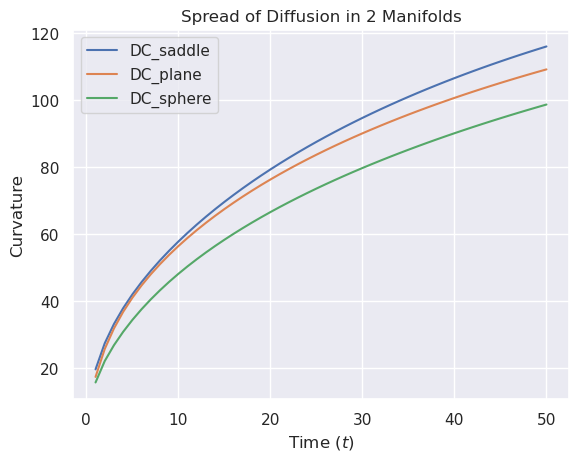
\includegraphics{index_files/figure-latex/..-nbs-experiments-2c3-are-kernels-zeitgeibers-fig-spread-of-diffusion-2d-output-1.png}

}

\caption{\label{fig-spread-of-diffusion-2d}Spread of Diffusion in 2
Manifolds}

\end{figure}%

\textsubscript{Source:
\href{https://professorwug.github.io/diffusion-curvature//Users/boreas/Pumberton/Workshop/21-SUMRY-Curvature/diffusion-curvature/nbs/experiments/2c3-are-kernels-zeitgeibers.ipynb.html\#cell-fig-spread-of-diffusion-2d}{Standard
libraries}}

\section{Conclusion}\label{conclusion}

\section*{References}\label{references}
\addcontentsline{toc}{section}{References}

\phantomsection\label{refs}
\begin{CSLReferences}{0}{1}
\vspace{1em}

\end{CSLReferences}



\end{document}
